\ The planned research schedule is heavily weighted on computational tasks. 
Bridgman will be the main high performance computer (HPC) utilized for analysis. 
Savio at UC-Berkley will be used to run Coeus for ETA-2 and ETA-SPNS. 
Due to the long nature of SAMPLER runs, the original ETA will be analyzed first on Bridgman. 
Figures \ref{fig:Cal1} to \ref{fig:Cal3} summarize a weekly schedule. 
The analysis periods are filled with many sub-tasks (plotting, $\chi^{2}$, running into errors, ect.)

\begin{figure}[ht]
	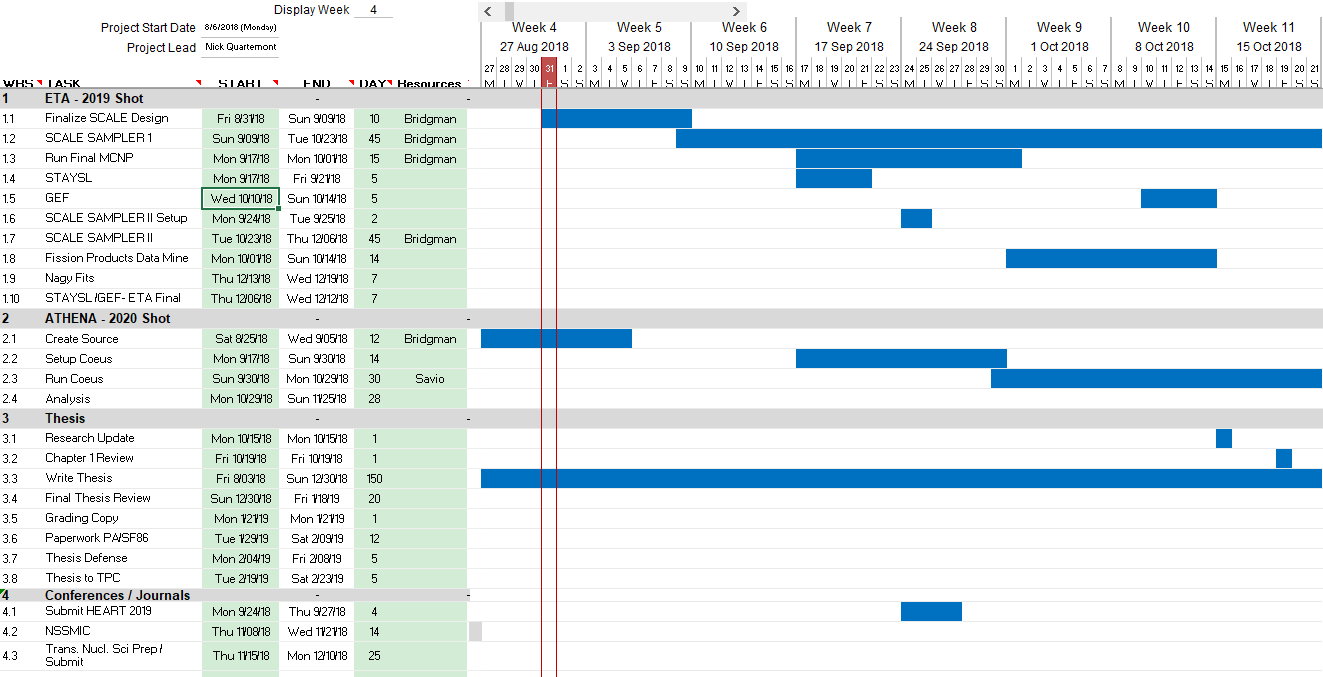
\includegraphics[width=\linewidth]{Figures/Chapter4/Cal1.png}
	\caption{Research schedule part 1}
	\label{fig:Cal1}
\end{figure} 

\begin{figure}[ht]
	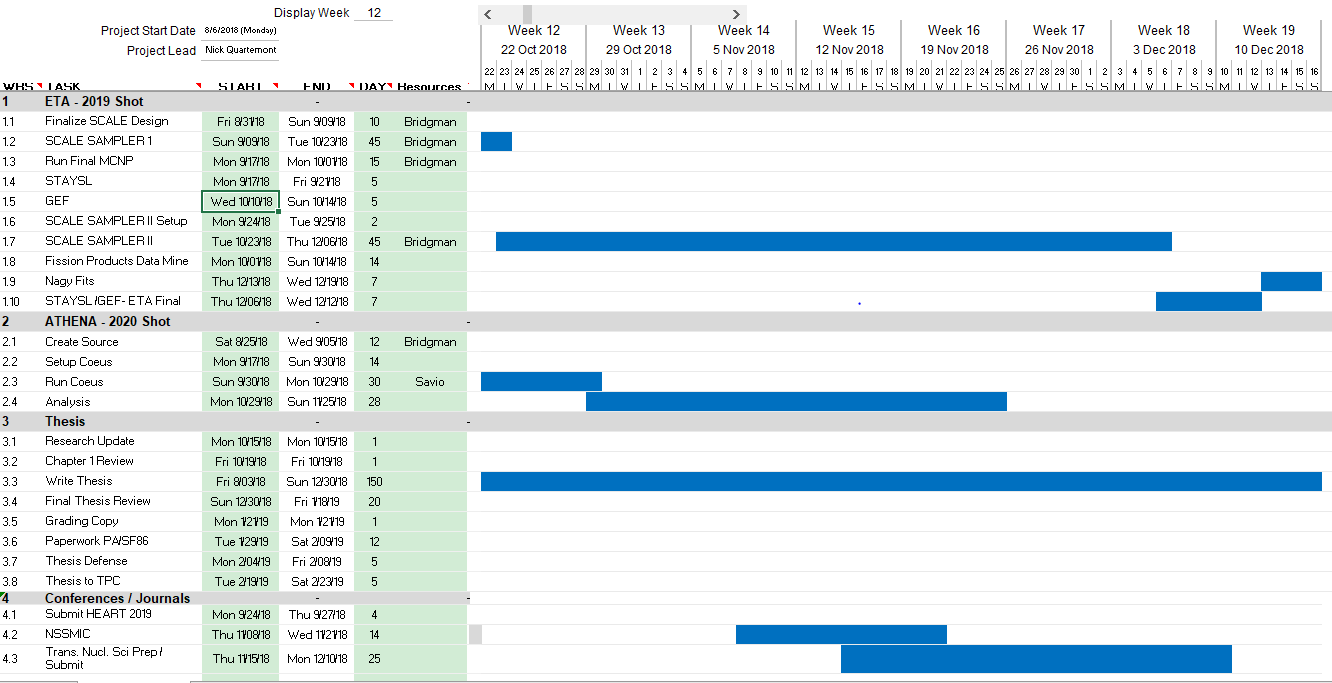
\includegraphics[width=\linewidth]{Figures/Chapter4/Cal2.png}
	\caption{Research schedule part 2}
	\label{fig:Cal2}
\end{figure} 
\begin{figure}[ht]
	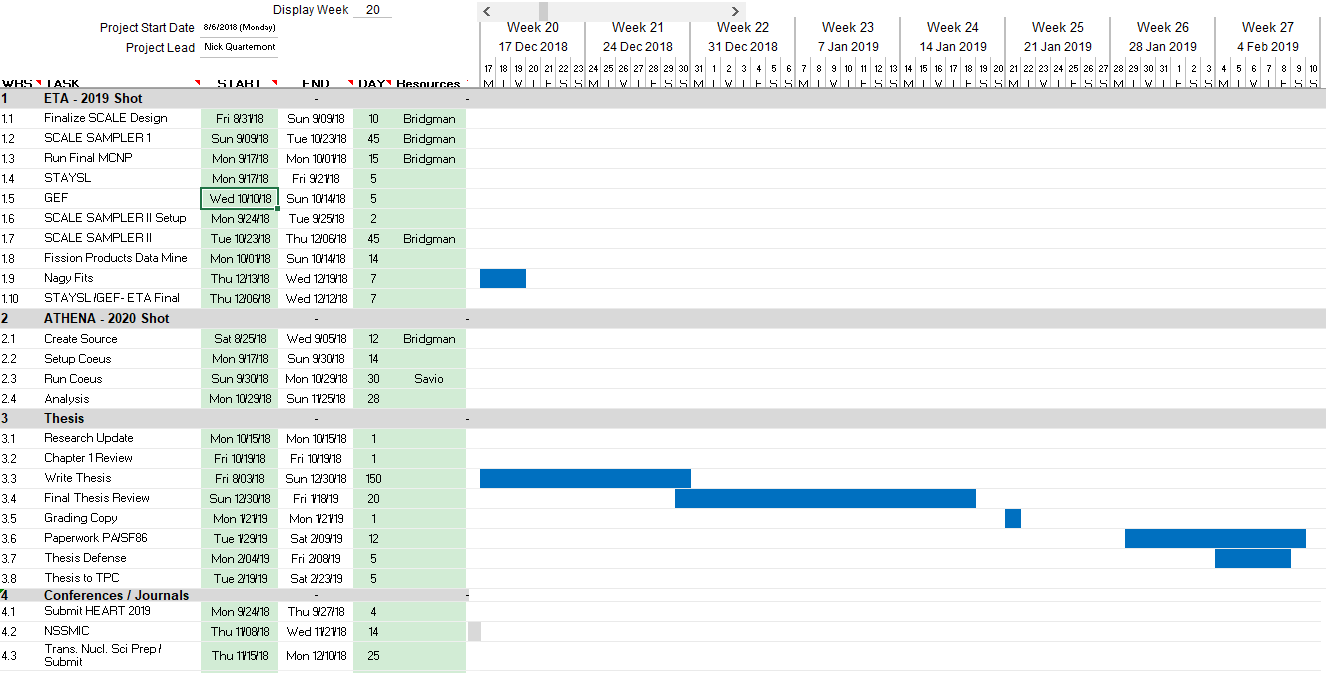
\includegraphics[width=\linewidth]{Figures/Chapter4/Cal3.png}
	\caption{Research schedule part 3}
	\label{fig:Cal3}
\end{figure} 
